\chapter{\sysname{} Design}
\label{sec:system-design}

In this section, we present an overview of \sysname{}. The primary goal of
\sysname{} is to enable applications with the ability to adapt its communication
in a guided manner.

\section{Challenges}
\label{sec:challenges}

\noindent There are four challenges in realizing \sysname{}.

\para{C1: Diverse application and data:} As discussed in~\autoref{sec:bat}, the
best adaptation scheme is often application- and context-specific
optimizations. It becomes important to separate individual application logic
from specific degradation strategy as well as adaptation mechanism.

\para{C2: No analytical solutions:} Unlike SQL queries whose demand and accuracy
can typically be estimated using analytical models~\cite{cormode2012synopses},
many of our streaming applications are dealing with unstructure data using
either use blackbox operations (such as H.264 encoding) or non-linear operators
(such as thresholding). The impact of these degradations is not immediately
available.

\para{C3: Multi-dimensional exploration:} Real-world applications typically have
more than one tunable parameters; leading to a combinatorial space for
exploration. In addition, these parameters are not necessarily orthognal.  The
optimal degradation strategies may only be achievable when more than one
degradation is in effect.

\para{C4: Runtime adaptation at application layer:} Although recent work on
resource reservation makes it possible to guarantee quality of service with new
IP or MAC layer protocols in LAN (e.g. TSN~\cite{johas2013heterogeneous}), we
target at WAN analytics where most of the infrastructure is owned by others and
shared among many users. An application-layer solution is in favor to those that
require special hardware or software upgrade.

\section{System Architecture}
\label{sec:architecture}

\begin{figure*}
  \centering
  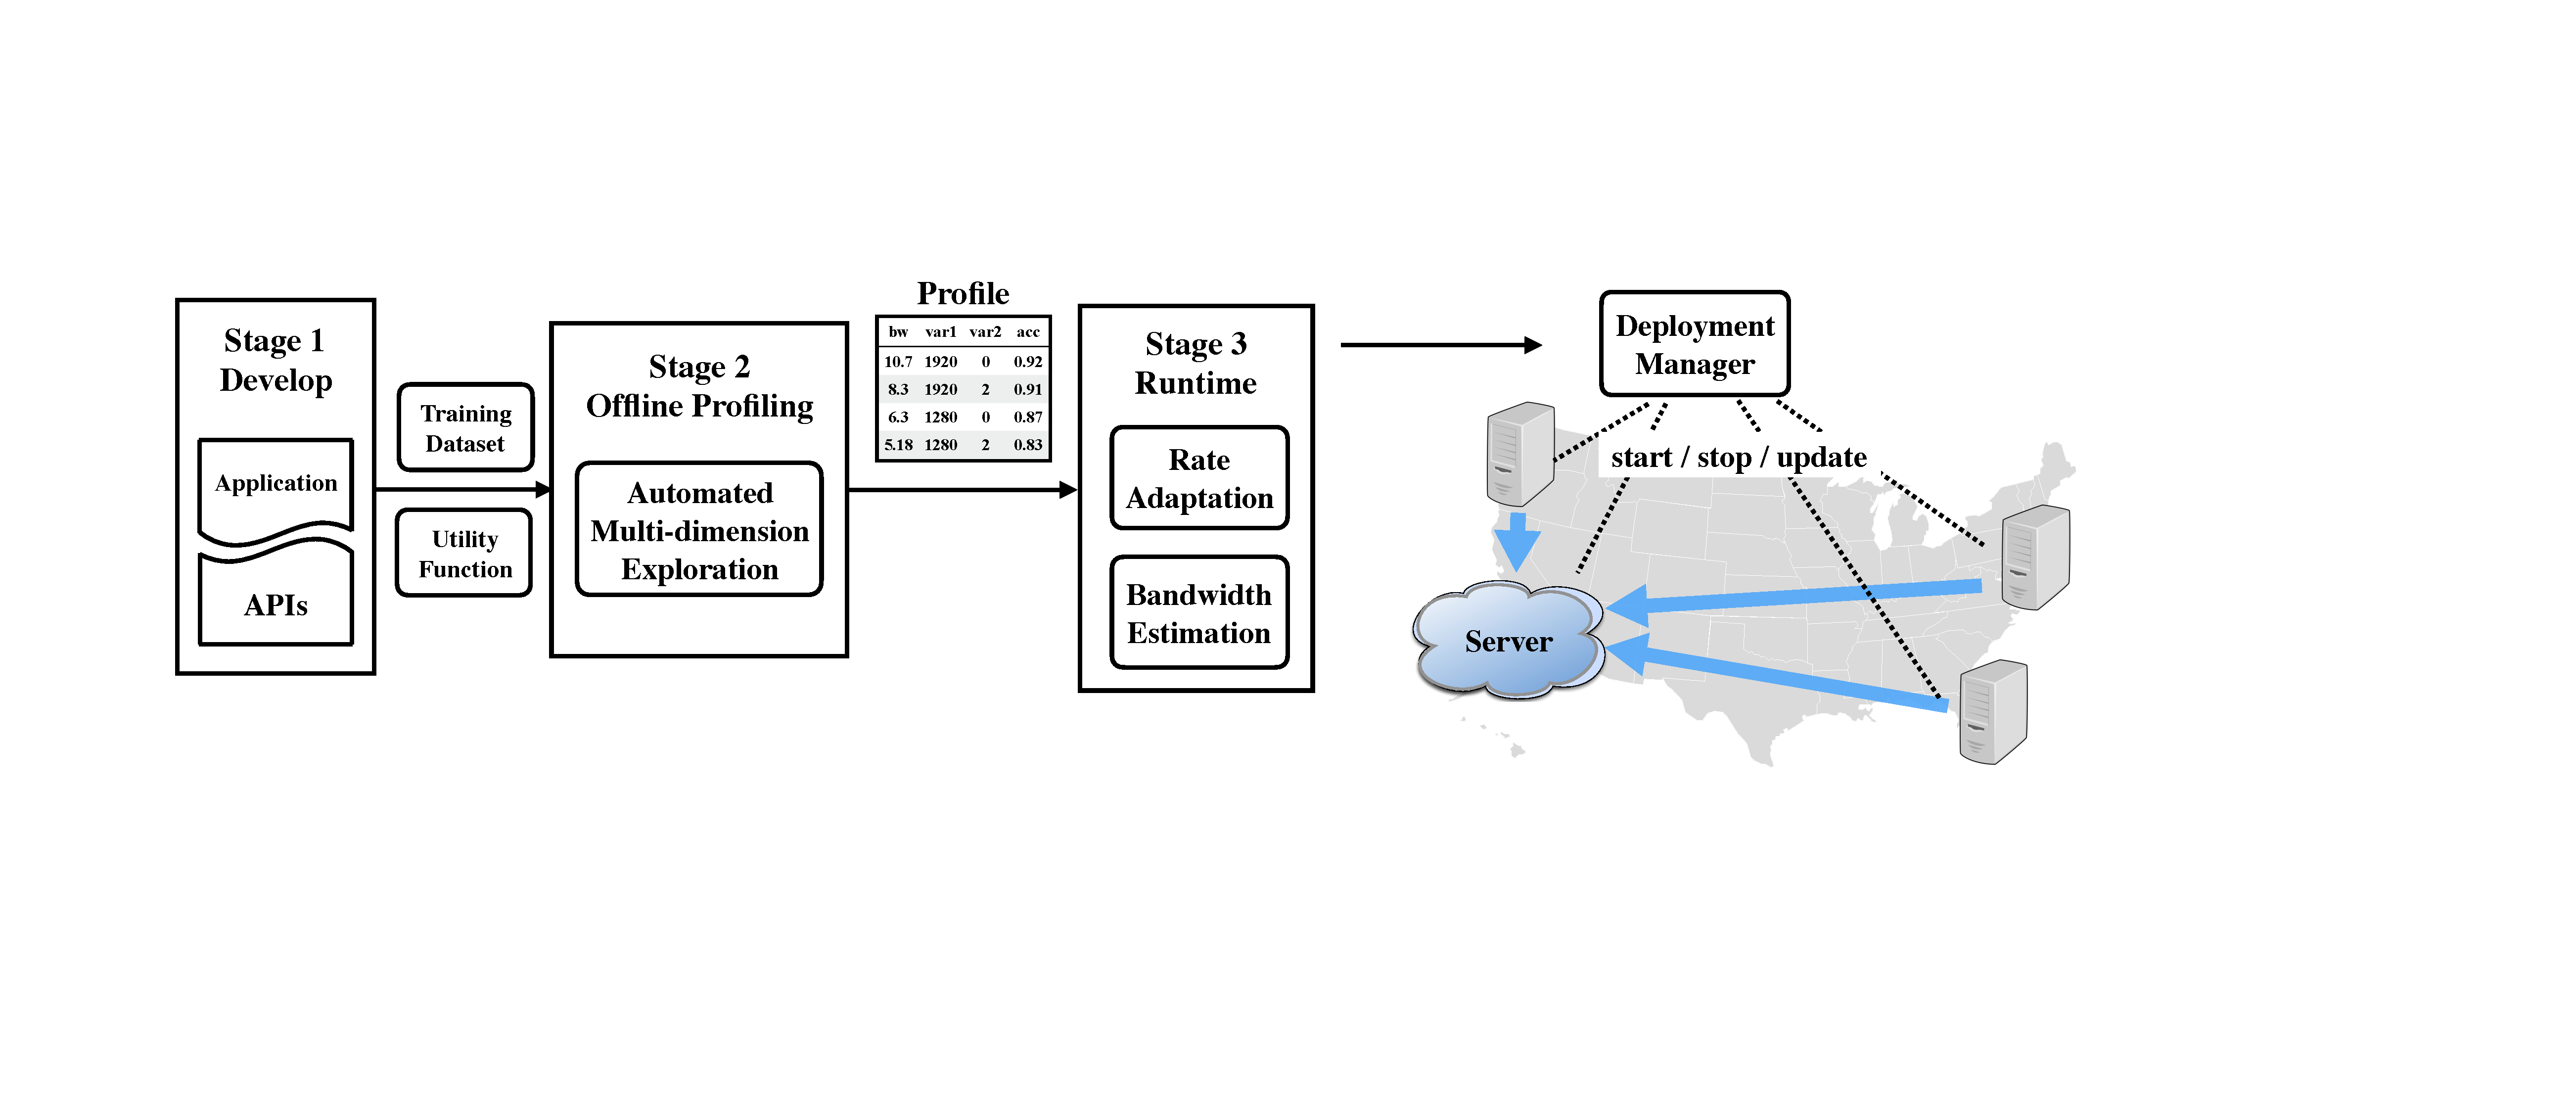
\includegraphics[width=\linewidth]{figures/arch.pdf}
  \caption{\sysname{} Overview.}
  \label{fig:overview}
\end{figure*}

To address the aforementioned challenges, \sysname{}'s solution is split into
four parts (\autoref{fig:overview}).

\para{Programming abstraction:} Applications are modelled as a directed acyclic
graph (DAG) of computation and we propose a novel set of \texttt{maybe}
operators to express the specification of degradation. Our propose APIs do not
require developers to be exact on the quantity; integrating this into existing
applications requires minimal effort (\autoref{sec:prog-abs}).

\para{Automatic multi-dimensional profiling:} Our system automatically explores
the parameter space to generate a Pareto-optimal degradation strategy with a
multi-dimensional exploration. We also report our experience and findings about
degradation operations (\autoref{sec:profiling}).

\para{Runtime Adaptation:} Finally the streaming application is deployed with a
wide-area orchestration manager. At runtime, our system generates additional
modules that acts as the control plane to adapt the application execution. The
control plane performs bandwidth estimation, congestion monitoring and
adaptation. It uses the profile generated from the second stage and adjust the
level of degradation (\autoref{sec:adaptation}).

\section{System Design}
\label{sec:system-design}

In this section, we dive into each component of \sysname{}; we focus on
degradation and adaptation, rather than being verbose on every component.

Applications in \sysname{} are composed by connecting a set of operators to form
a dataflow processing graph. Our system provides basic set of APIs such as
\texttt{map}, \texttt{filter}, \texttt{window} (\autoref{tab:operators}). The
normal operators are similar to existing stream processing systems; our
contribution is the set of APIs to allow the specification of degradation
operations for bandwidth-accuracy trade-off.

\begin{table*}
  \centering
  \begin{tabular}{ c r l }
    \toprule
    \multirow{7}{*}{Normal Operators}
    & \textit{map}(f: I $\Rightarrow$ O) & Stream<I> $\Rightarrow$ Stream<O> \\
    & \textit{filter}(f: I $\Rightarrow$ bool) & Stream<I> $\Rightarrow$
                                                 Stream<I> \\
    & \textit{skip}(i: Integer) & Stream<I> $\Rightarrow$ Stream<I> \\
    & \textit{sliding\_window}(count: Integer, f: Vec<I> $\Rightarrow$ O) & Stream<I> $\Rightarrow$
                                                                            Stream<O> \\
    & \textit{tumbling\_window}(count: Integer, f: Vec<I> $\Rightarrow$ O) & Stream<I> $\Rightarrow$
                                                                             Stream<O> \\
    & \textit{timed\_window}(time: Duration, f: Vec<I> $\Rightarrow$ O) & Stream<I> $\Rightarrow$
                                                                          Stream<O> \\
    & ... & ... \\
    \midrule
    \multirow{4}{*}{Degradation Operators}
    & \textit{maybe}(knobs: Vec<T>, f: (T, I) $\Rightarrow$ I) & Stream<I> $\Rightarrow$
                                                                 Stream<I> \\
    & \textit{maybe\_skip}(knobs: Vec<T>) & Stream<I> $\Rightarrow$ Stream<I> \\
    & \textit{maybe\_downsample}(knobs: Vec<(Integer, Interger)>) & Stream<Image> $\Rightarrow$ Stream<Image> \\
    & ... & ... \\
    \bottomrule
  \end{tabular}
  \caption{A comparison between normal stream processing operators and our
    degradation operators. Vec<T> represents a list of elements of type
    T. Option<T> indicates an element of type T can be absent. Notice the type
    constrain on the \texttt{maybe} function while \texttt{maybe\_map} relaxes
    it.}
  \label{tab:operators}
\end{table*}

\subsection{Degradation Operators}
\label{sec:prog-abs}

We first consider a strawman solution: manual policies for
degradation. JetStream~\cite{rabkin2014aggregation} offers an example: ``if
bandwidth is insufficient, switch to sending images at 75\% fidelity, then 50\%
if there still isn't enough bandwidth. Beyond that point, reduce the frame rate,
but keep the images at 50\% fidelity.'' We identify the following issues with
this approach.

\para{Lack of precision:} These policies are often developer heuristics and
rarely backed up by measurements. First, there is no direct association of the
application accuracy with the 75\% fidelity configuration. Besides, their impact
on the data size is also not trivial.  While it seems intuitive that the level
of degradation will affect the data size, the precise impact is not always
straightforward. For example, one might think that reducing the frame rate by
50\% will half the data rate. When video encoding is employed, the inter-frame
difference will increased (P-frame size) when the frame rate is reduced. This
leads to a larger data size for each frame. \autoref{fig:h264} illustrates this
complex relationship with an example of H.264 encoding under four different
frame rates.

\para{Not scalable:} The strawman solution quickly leads to too many policies
when multiple degradation operations are involved or a fine-grained control is
desired. This manual process becomes tedious and error-prone. When too few rules
are provided, the application may oscillate between two rules: one that's too
aggressive (always faces insufficient bandwidth) and one that's too
conservative.

\begin{figure}
  \centering
  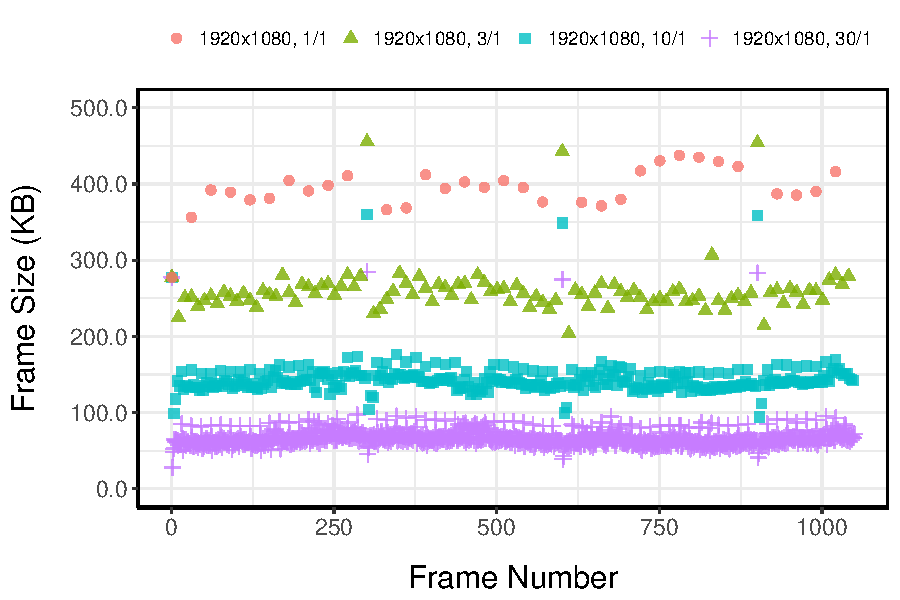
\includegraphics[width=\columnwidth]{figures/h264.pdf}
  \caption{H.264 requires more information per frame when the frame rate is
    reduced.}
  \label{fig:h264}
\end{figure}

\vspace{0.5em}

When using the above strawman solution, developers are forced to manually study
and measure the impact of individual degradation policy, prohibiting its wide
adoption in practice.

On the other extreme of the design spectrum, a completely developer-free
solution is not practical. While static analysis has been shown to optimize
application execution adaptively in a certain context~\cite{chun2011clonecloud},
they do not work well in our dataflow programming model. Static analysis is
prone to false positives: exploring wrong or unnecessary parameters. For
example, when the application is configured to generates statistics with a
\texttt{timed\_window} operation, static analysis may falsely detect the
duration parameter and alter the behavior of the application in an unexpected
way. Also, as we will illustrate in~\autoref{sec:profiling}, with each
introduced parameter, the profiling time increases drastically as all parameters
pose a combinatorial space.

Our system take a middle ground between these two extremes: developers use a
novel \texttt{maybe} API to annotate degradation operations without being exact
on the values. Think of these APIs as hints from developers: this operation,
when in use, will likely reduce the data size and affect the data fidelity;
however the exact impact is not clear.

The basic form of \texttt{maybe} operator takes two arguments: a knob and a
degradation function (see \autoref{tab:operators}). The knob indicates different
degradation levels; the function performs the actual degradation operation with
a configurable level. We restrict the type signature of the function that this
API can accept: $f(T, I) \Rightarrow I$. That is, the degradation function
should not alter the type of the stream. While this might seem a strong
restriction, when combined with \texttt{map} operator, the system is still
expressive enough. We describe our implementation and usage
in~\autoref{sec:implementation}.

\begin{sloppypar}
  Based on the \texttt{maybe} primitive, one can implement wrappers for common
  degradation operations. For example, \texttt{maybe\_skip} will optionally
  subsample a stream; and \texttt{maybe\_downsample} can adjust the image
  resolution to a configured target. With this API, the example mentioned
  earlier can now be implemented as follows:
\end{sloppypar}

\begin{lstlisting}
   let app = Camera::new((1920, 1080, 30))
      .maybe_downsample(vec![(1600, 900), (1280, 720)])
      .maybe_skip(vec![2, 5])
      .map(|frame| frame.show())
      .compose();
\end{lstlisting}

This snippet first instantiate a \texttt{Camera} source, which is a
\texttt{Stream<Image>} with 1920x1080 resolution and 30 FPS. Two degradation
operations are chained after the source: one that downsample the resolution to
either 1600x900 or 1280x720; the other skip the frame with a parameter of 2 or
5, resulting in 30/(2+1)=10 FPS or 30/(5+1)= 6 FPS. After the degradation,
images are shown on the display. In practice, further processing operators can
be chained.

While the API itself has simplified the specification of degradation, the exact
amount has to be known for precise rate adjustment at runtime. We then turn to
the second stage of our system that performs automatic profiling.

\section{Multi-dimensional Profiling}
\label{sec:profiling}

The goal of our profiling stage is to explore the bandwidth-accuracy trade-off
and generate a \textit{profile} that is Pareto-optimal.

We first define terms and notations we will use. Each \texttt{maybe} operator
within an application corresponds to a knob $k$. Suppose the application has $n$
knobs, their combination forms a configuration $c = [k_{1}, k_{2},
... k_{n}]$. The set of all configurations $\mathbb{C}$ is the space that our
profiling system need to explore.

There are two mappings that we are particularly interested: a mapping from a
particular configuration to its bandwidth requirement $B(c)$ and the accuracy
measure $A(c)$. The Pareto-optimal set $\mathbb{P}$ can then be defined
(\autoref{eq:pareto}): for all $c \in \mathbb{P}$, there is no alternative
configuration $c'$ that requires less bandwidth while giving a higher accuracy.

{\small
\begin{equation}
  \mathbb{P} = \{ c \in \mathbb{C} : \{ c' \in \mathbb{C}: B(c') < B(c),
  A(c') > A(c) \} = \varnothing\}
  \label{eq:pareto}
\end{equation}
}%

\begin{table}
  \centering
  \begin{tabular}{r l}
    \toprule
    \textbf{Symbol} & \textbf{Description} \\
    \midrule
    $n$ & number of degradation operations \\
    $k_i$ & the \textit{i}-th degradation knob \\
    $c = [k_{1}, k_{2}, ... k_{n}]$ & one specific configuration \\
    $\mathbb{C}$ & the set of all configurations \\
    \midrule
    $B(c)$ & bandwidth requirement for $c$ \\
    $A(c)$ & accuracy measure for $c$ \\
    $\mathbb{P}$ & Pareto efficienct set \\
    \bottomrule
  \end{tabular}
  \caption{Notations used in profiling.}
  \label{tab:notations}
\end{table}

Since there is often no closed form relation for $B(c)$ and $A(c)$, our system
takes a data-driven approach: with a representative dataset and an
application-specific utility function, our system evaluates each configuration
for their bandwidth demand and accuracy degradation. The degradation could
either be measured against the groundtruth; or in the case when labelled dataset
is not available, the system uses the reference results when all degradations
are turned off.

% \begin{figure}
%   \centering
%   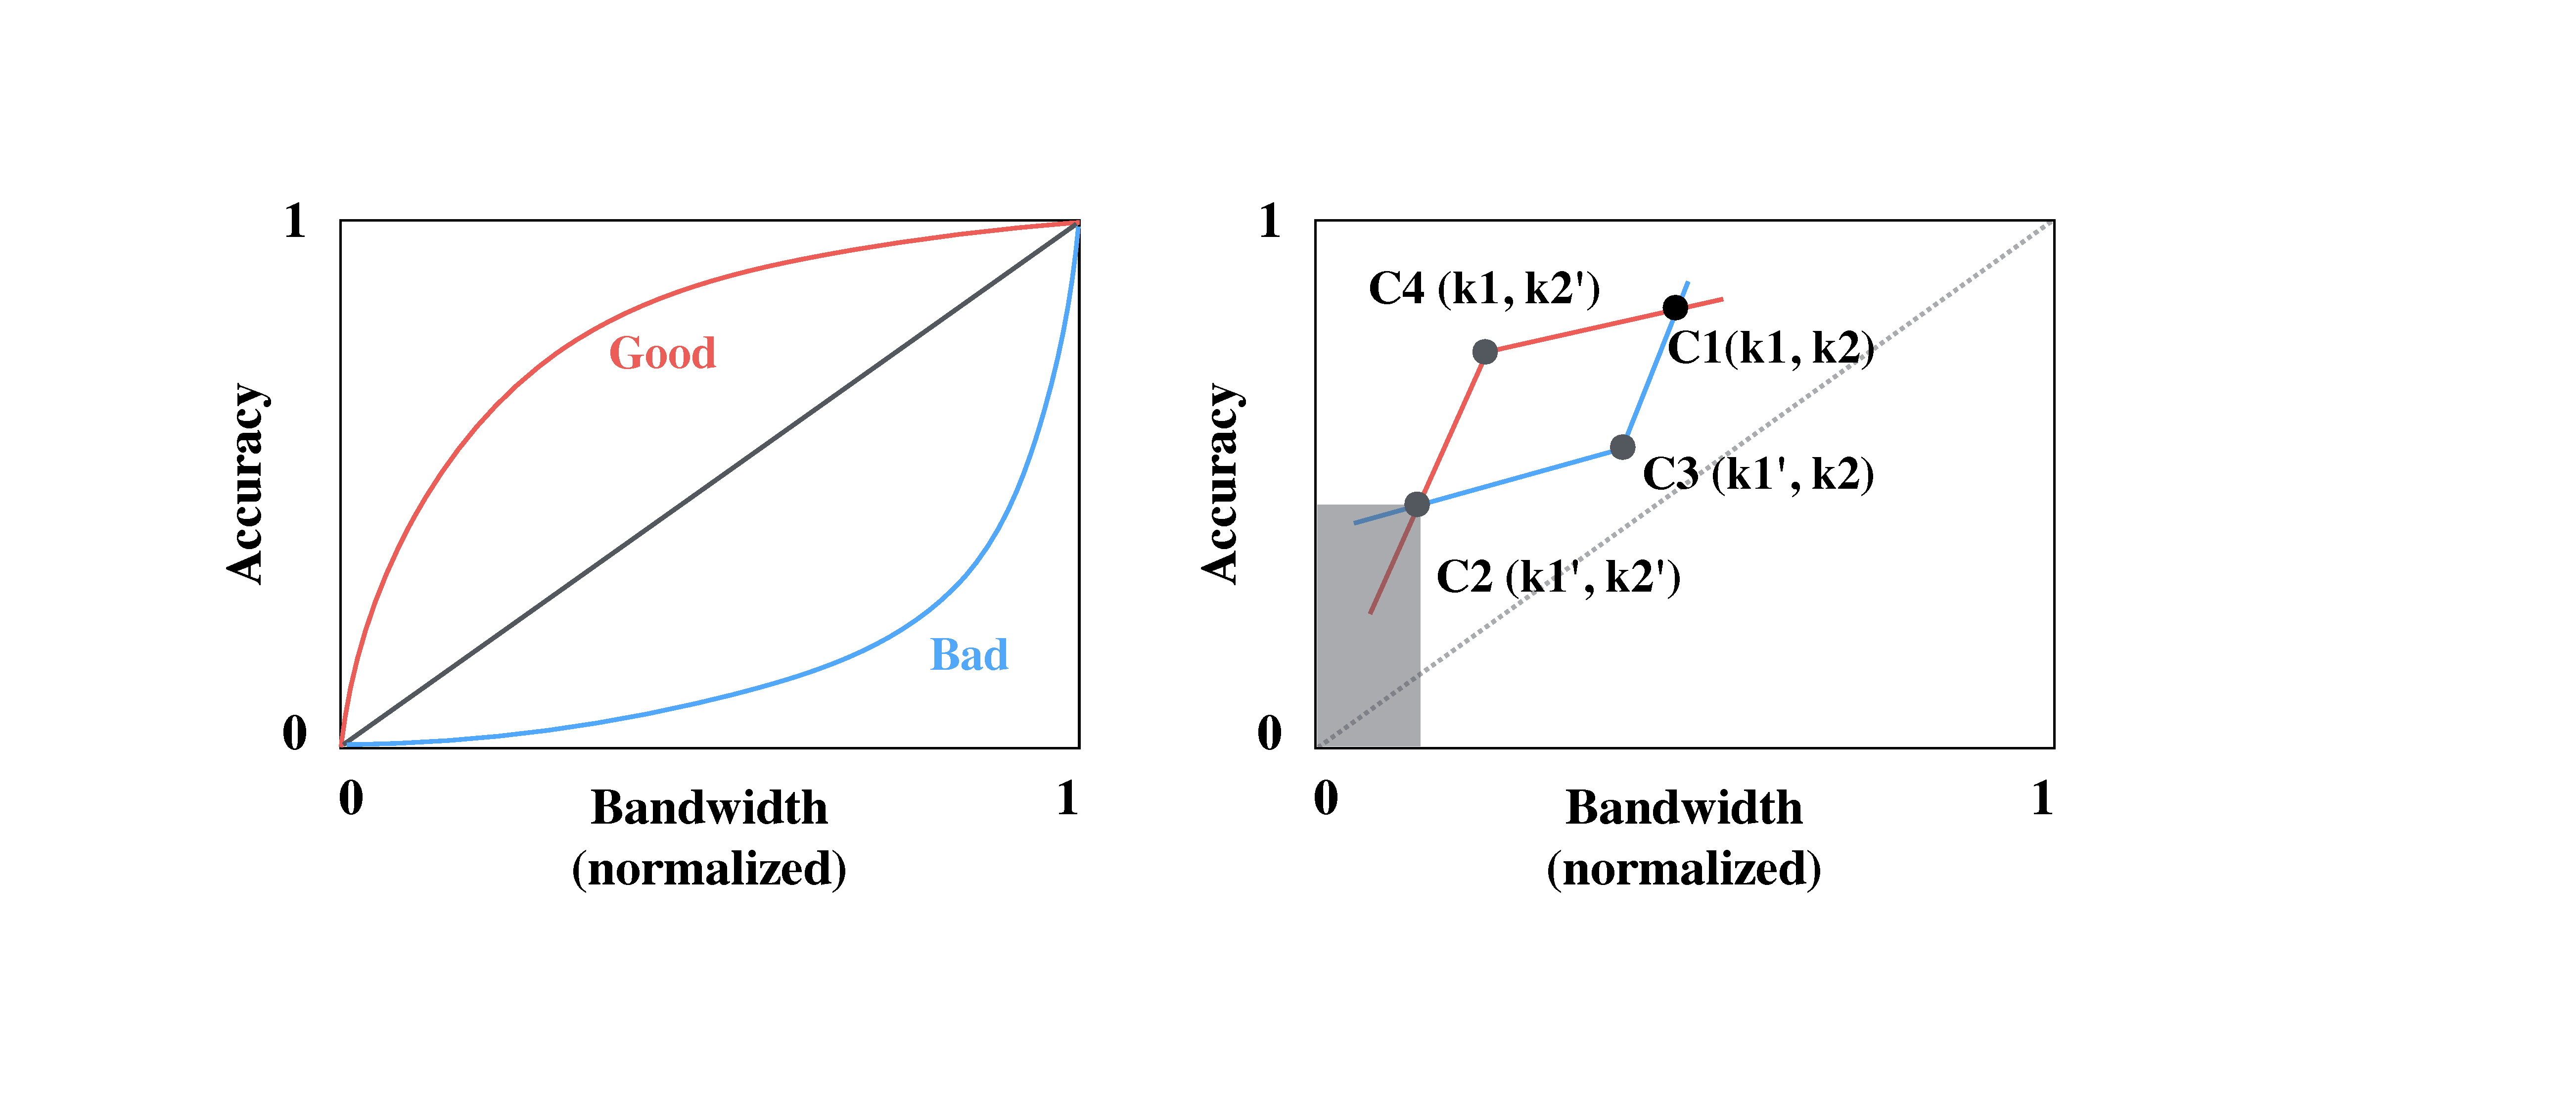
\includegraphics[width=\columnwidth]{figures/degrade.pdf}
%   \caption{Illustration on the behavior of different degradation operations.}
% \end{figure}

When only one knob is involved, we can represent its impact using
bandwidth-accuracy curve (\autoref{fig:bat} left) and quantify the effect with
the area under the curve (AUC). Each curve consists of the point with coordinate
$(B(c), A(c))$ when configuration $c$ is used. The straight line from (0, 0) to
(1, 1) splits the space into two parts. If a degradation's profile lies above
this line, it indicates that this operation can be effective for the goal of
saving bandwidth while minimizing accuracy drop. For degradation operations
that's below the straight line, much of the data information is gone even at
minor bandwidth drop. The Pareto-optimal strategy is the profile that has a
maximal AUC.

While $B(c)$ and $A(c)$ can be monotonic along individual dimension. When
combined, it poses complex behavior. The right half illustrates
\autoref{fig:bat} illustrates it.

While the complexity prohibits further analytical analysis of the degradation
behavior, in practice, several techniques can make the problem tractable. First,
Exploring these configurations is an embarrassingly parallel task. The profiling
can be made trivially parallel. Besides, when the degradation level increases or
when multiple degradation operations are in effect, the amount of data as well
as the computational complexity are also dramatically reduced.  Moreover,
developers can specify a lower bound on the accuracy and the profiling can stop
searching the space that is worst than a known configuration (such as the gray
area in \autoref{fig:bat}).

\subsection{Runtime Adaptation}
\label{sec:adaptation}

\begin{figure}
  \centering
  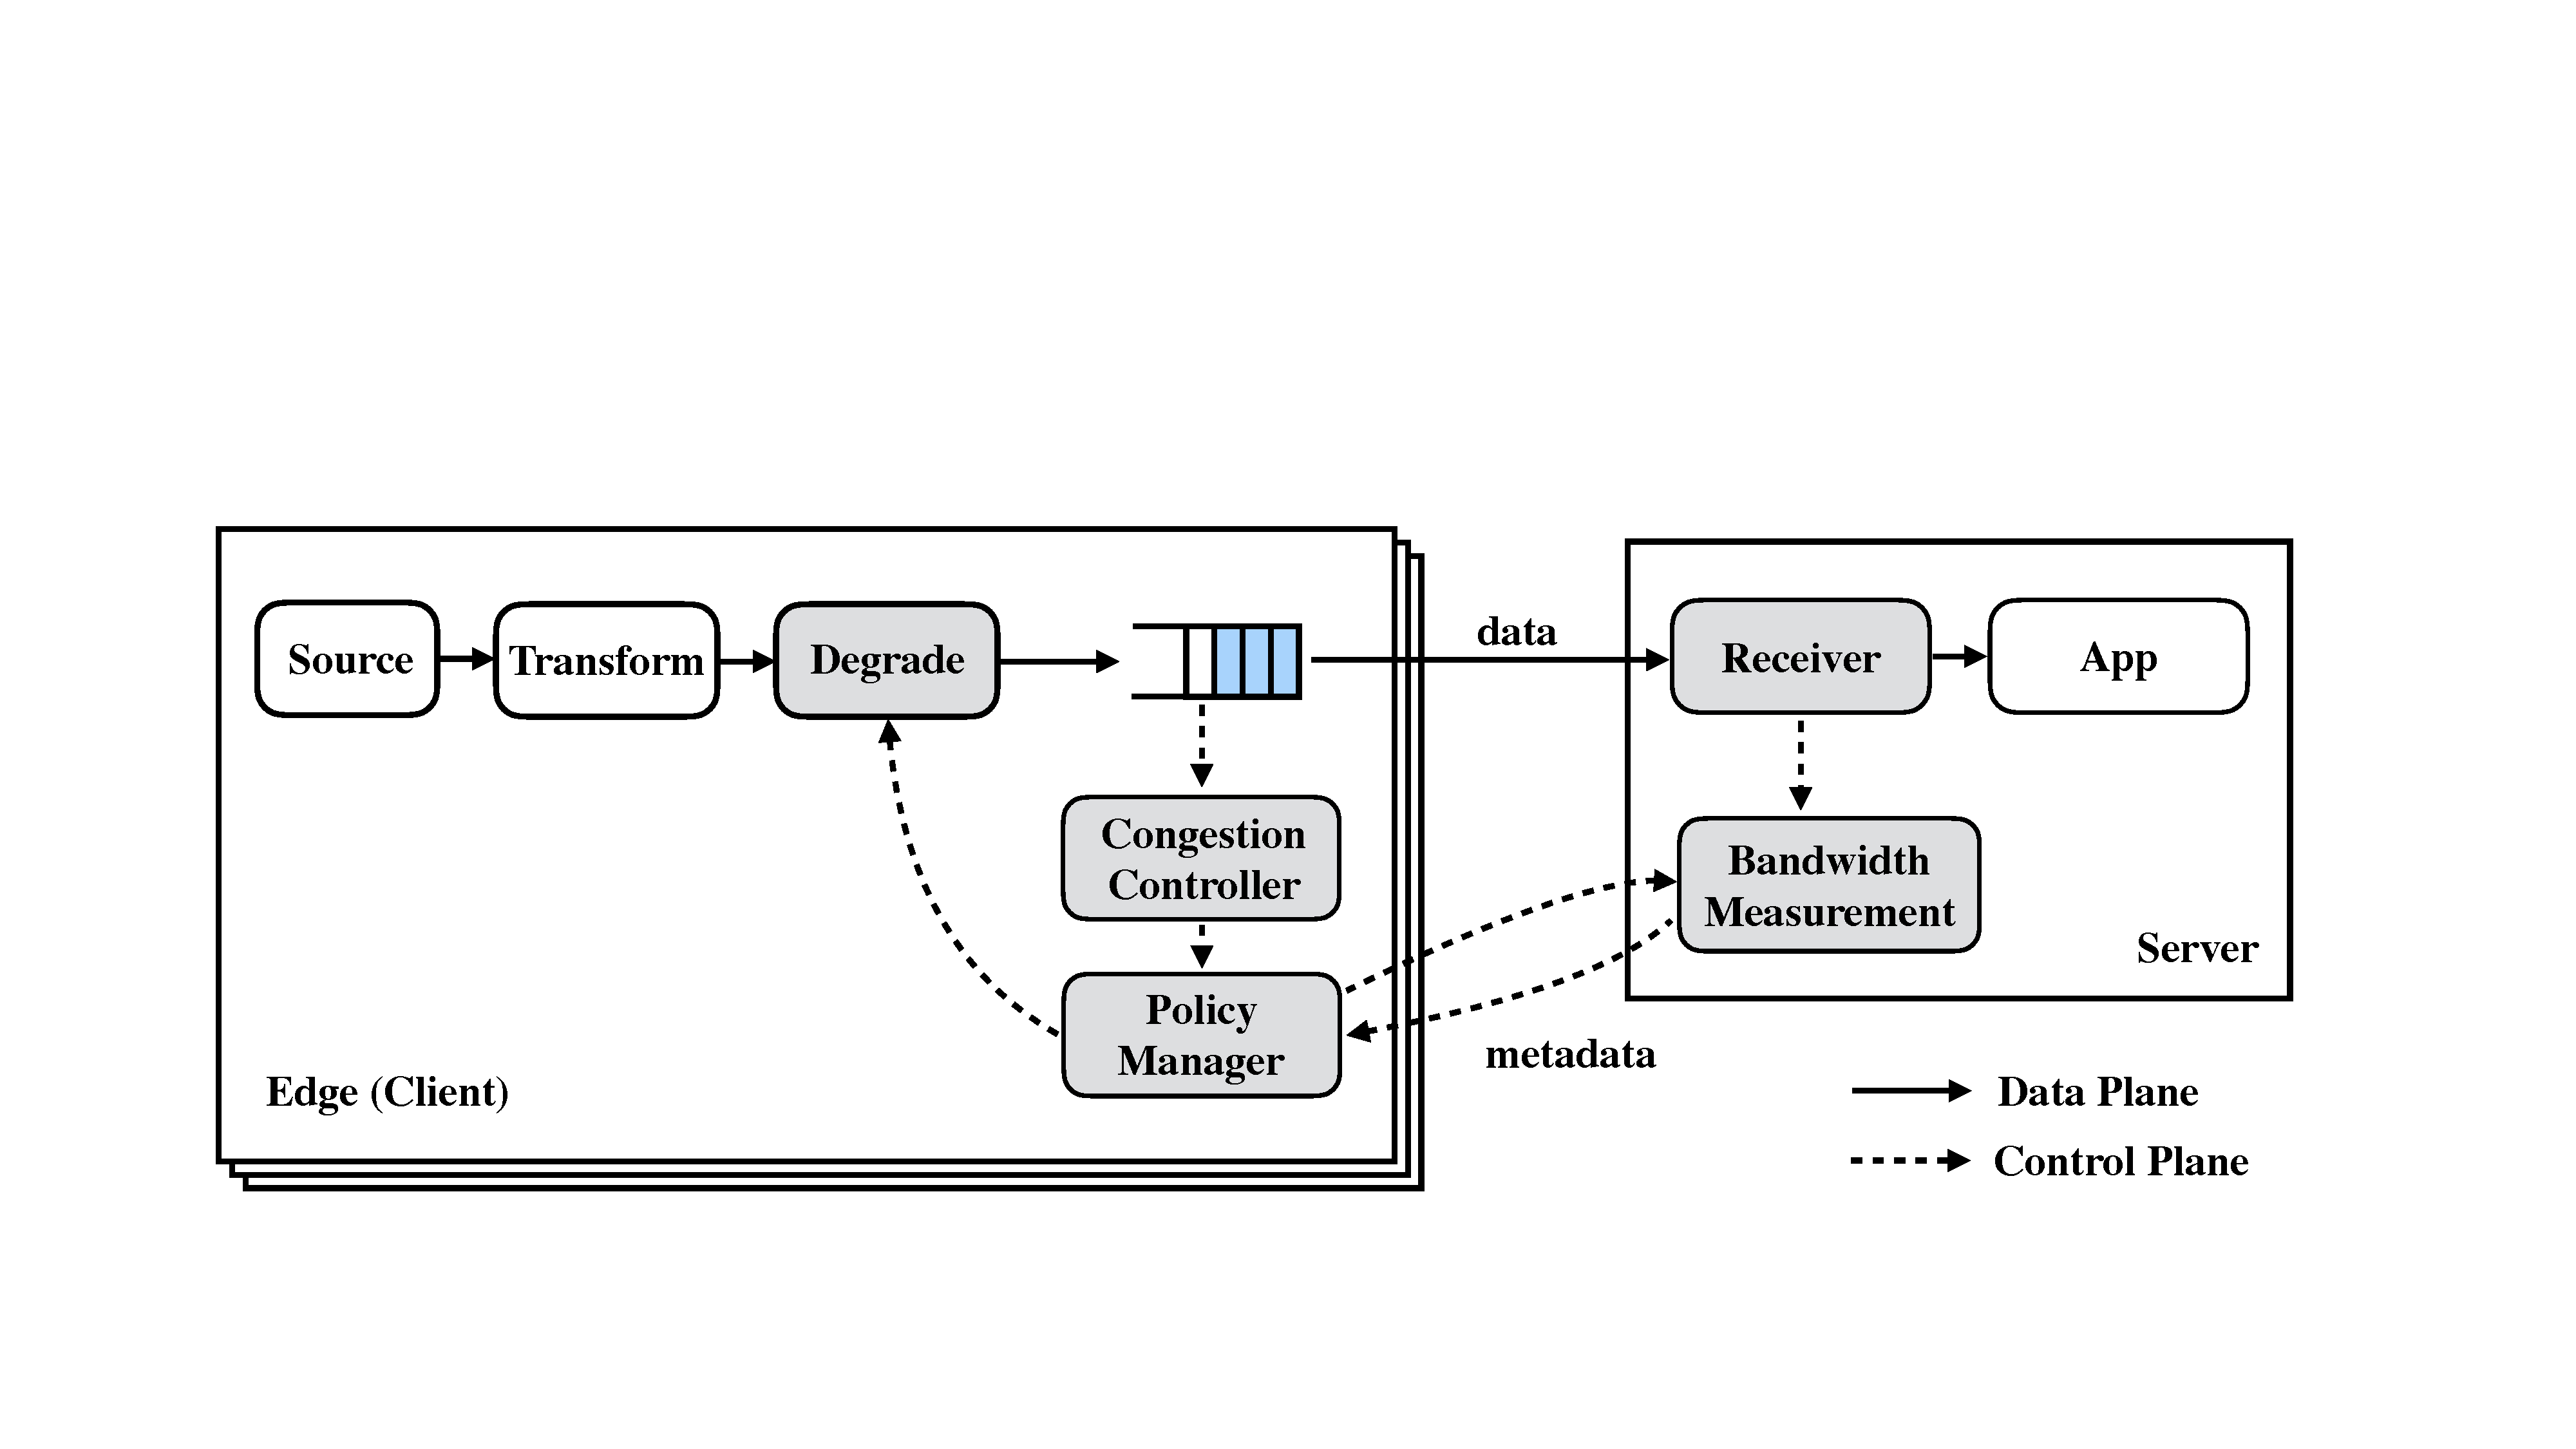
\includegraphics[width=\linewidth]{figures/runtime.pdf}
  \caption{Runtime adaptation system architecture. The grey components are what
    \sysname{} provides.}
  \label{fig:runtime}
\end{figure}

At runtime, the user program is automatically converted to a client half and
server half; and \sysname{} abstracts the communication as well as rate
adaptation. \autoref{fig:runtime} shows our runtime architecture.

\para{Object-level queue:} The queue bridges data generation and
the network capacity. It transmits data as fast as the network can handle and
detects congestion when the queue grows.

\para{Congestion controller:} Our first prototype used the queue length as a
signal for congestions, this turns out to be a bad match as the degradation
operation may change object arrival rate (e.g.\,lower frame rate for video). Our
next version uses data size, but it also leads to long latency when the
degradation changes individual object size (e.g.\,lower resolution). Our current
design uses an adaptive size: given current configuration and the profile, the
queue learns the desired data generation rate (bps), and with a user configured
latency, the queue derive the congestion watermark.

\para{Bandwidth Measurement:} The receiver delivers the received data to
application. In the meantime, it measures the effective throughput between each
client-server pair as an indication of current bandwidth~\cite{iperf}. To avoid
spikes in the bandwidth measurement, exponential smoothing is employed. While
the receiver performs bandwidth measurement every second, it does not send the
information back to each client.  avoid unnecessary communication, the client
requests the measurement only when congestion is detected.

\para{Policy Manager:} Upon receiving signals from congestion controller, it
performs an RPC request to the server for current bandwidth measurement. With
the learned profile, it determines the degradation level and start the actual
degradation strategy. The bandwidth specification in the learned profile is the
required bandwidth, the policy manager usually takes a conservative approach:
using a constant rate ALPHA to adjust the available bandwidth. When the
congestion is resolved, the policy manager gradually reduce the degradation
level (additive increase phase).

\para{Degrade:} The actual degradation operation is rather simple. Operators
based on the \texttt{maybe} API supports a \texttt{set} function that would
change the internals of the operator. The \texttt{set} function is invoked when
degradation is needed.

%% {Interaction with TCP:} Our runtime system follow the tuning guide
%% \cite{tierney2001tcp} to adjust the send buffer.

%%% Local Variables:
%%% mode: latex
%%% TeX-master: "sigcomm2017"
%%% End:

%%% Local Variables:
%%% mode: latex
%%% TeX-master: "thesis"
%%% End:
